%% ----------------------------------------------------------------
%% AppendixA.tex
%% ---------------------------------------------------------------- 
\chapter{Get Started with \emph{RiskVis}} \label{Chapter:AppendixA}

In order to evaluate how well test users can use functionalities in RiskVis, I have designed four different tasks. This document is not a thorough user manual that introduces everything in RiskVis but a tutorial that helps new users complete given tasks as quickly as possible.

\section{Data Source Connection}

RiskVis is a standalone application aiming at visualising data in the SAP Community Network (SCN) forum. If you have already installed the SCN forum database, you are welcome to download RiskVis via \url{http://users.ecs.soton.ac.uk/cx5g10/riskvis/riskvis_bin_20110909.zip}. Then set up database connection as follows:

\begin{enumerate}
	\item Unzip the file riskvis\_bin\_20110909.zip to any folder you like (suppose it's named YOURFOLDER); \\
	\item Execute YOURFOLDER/riskvis/bin/riskvis.exe to start the application; \\
	\item Select the Tools - Options menu item in the main menu; \\
	\item In the Miscellaneous - Data Source Configuration tab pane input your database connection parameters as well as the name of data tables, then click OK button to save (see \fref{Figure:0a_01}).
\end{enumerate}

\begin{figure}[!htb]
  \centering
  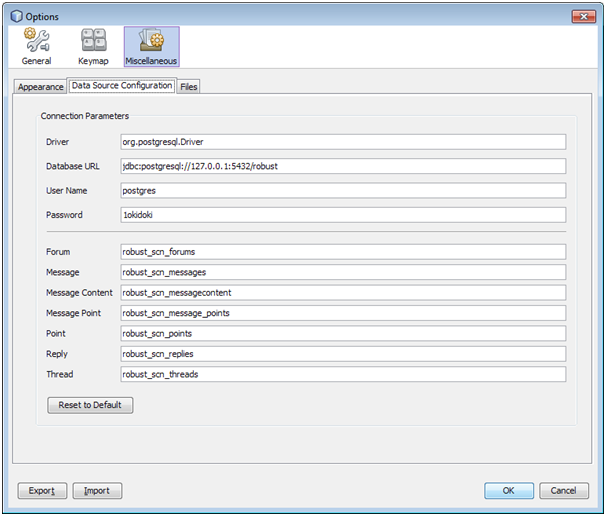
\includegraphics{0a_01}
  \caption{Data Source Configuration.}
  \label{Figure:0a_01}
\end{figure}

\section{Task A: Load Data and Open Collaborative Network}

\begin{enumerate}
	\item When RiskVis has been opened, you can see the Snapshot Explorer in left of the screen, as shown in \fref{Figure:0a_02}. If the tool fails to display it for some reason, you can open it manually from Window - Snapshot Explorer from the main menu (see \fref{Figure:0a_03}); \\
	\item In the Condition panel, do not change the drop-down list underneath the `Please choose a forum to analyse' label. Choose `2010', `August', and `1', respectively, as options for three drop-down lists underneath the `Please choose year, month, and duration' label. Then click the Load button. That means you want to load all data in the `Process Integration' forum during August 2010. As illustrated in \fref{Figure:0a_04}, the Load button becomes disabled until the snapshot data has been loaded. A progress bar in the bottom of the screen indicates the progress. It takes about 3 minutes to load this snapshot, please wait; \\
	\item Now click the left arrow button in top right corner of the Snapshot Explorer window to collapse it. Once the progress bar reaches 100\%, a new item will appear underneath the Condition panel of the Snapshot Explorer. Meanwhile, a collaborative network is automatically opened in the right of the screen, as shown in \fref{Figure:0a_05}. Notice that the Snapshot Explorer is in the left sliding side (red rectangle). \\
\end{enumerate}

\begin{figure}[!htb]
  \centering
  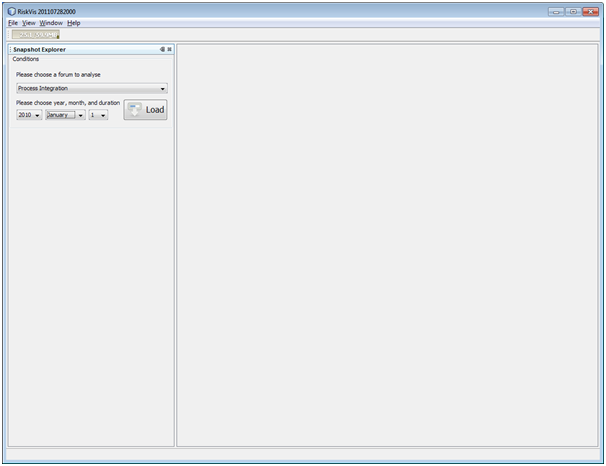
\includegraphics{0a_02}
  \caption{Initial Status of Snapshot Explorer.}
  \label{Figure:0a_02}
\end{figure}

\begin{figure}[!htb]
  \centering
  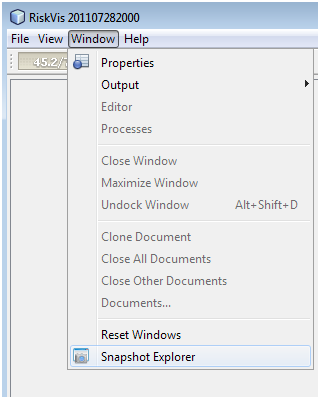
\includegraphics{0a_03}
  \caption{Open Snapshot Explorer from Main Menu.}
  \label{Figure:0a_03}
\end{figure}

\begin{figure}[!htb]
  \centering
  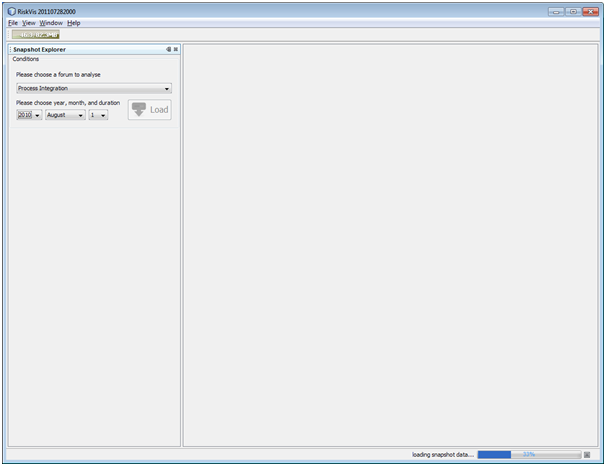
\includegraphics{0a_04}
  \caption{Loading Snapshot Data in `Process Integration' Forum during 08/10.}
  \label{Figure:0a_04}
\end{figure}

\begin{figure}[!htb]
  \centering
  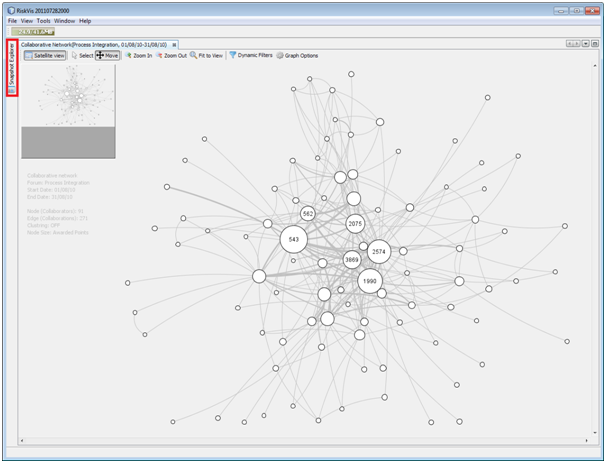
\includegraphics{0a_05}
  \caption{Collaborative Network of Snapshot (`Process Integration' Forum during 08/10) is Opened.}
  \label{Figure:0a_05}
\end{figure}

\section{Task B: Find the Most Important Collaborator}

\begin{enumerate}
	\item Suppose you have finished Task A, and have opened a Collaborative network as shown in \fref{Figure:0a_05}. Click the `Graph Options' button in the top right of the network. A new window will be opened in the right of the screen (see \fref{Figure:0a_06}); \\
	\item Find the node with the biggest size. It is the collaborator 543 in Figure 6, which indicates the collaborator 543 has the highest awarded points in the network; \\
	\item Choose another option called `Degree Centrality' for the drop-down list in the red rectangle of \fref{Figure:0a_06}. The graph will be refreshed and the node size is mapped to the degree centrality, as shown in \fref{Figure:0a_07}. Now you may see the biggest node is the collaborator 2574; \\
	\item Repeat the previous step with the other two options (betweenness centrality and closeness centrality) the for the drop-down list in the red rectangle of \fref{Figure:0a_07}. Please try it yourself. You may find the collaborator 2574 is still the biggest node. Now it is safe to conclude that the collaborator 2574 is the most important individual in the network.
\end{enumerate}

\begin{figure}[!htb]
  \centering
  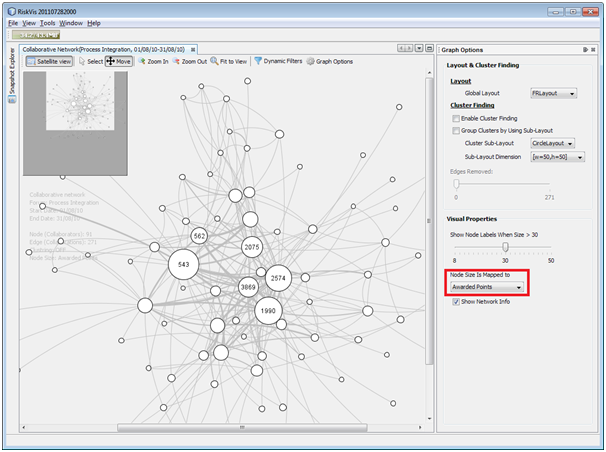
\includegraphics{0a_06}
  \caption{Open Graph Option Window of Collaborative Network.}
  \label{Figure:0a_06}
\end{figure}

\begin{figure}[!htb]
  \centering
  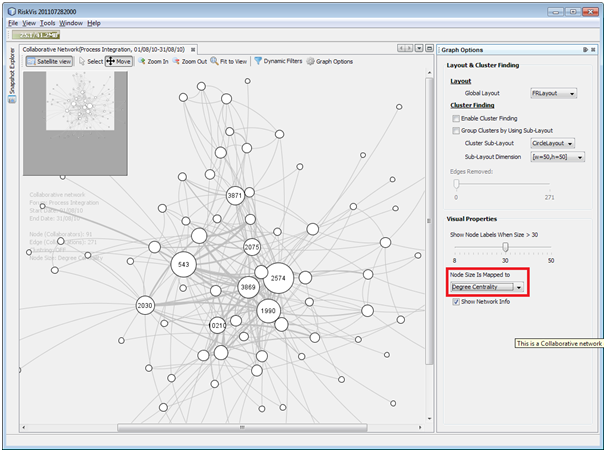
\includegraphics{0a_07}
  \caption{Node Size is mapped to Degree Centrality.}
  \label{Figure:0a_07}
\end{figure}

\section{Task C: Explore How Collaborations are distributed over Time}

\begin{enumerate}
	\item Suppose you have finished Task A and B, and have realised that the collaborator 2574 is the most important one in the network. In \fref{Figure:0a_07}, right click the node labelled 2574 to show the context menu, click the Goto Collaborator Centric Network menu item as shown in \fref{Figure:0a_08}; \\
	\item A new window will be opened in the main area of the screen as shown in \fref{Figure:0a_09}; \\
	\item Click the `Temporal Chart' button in the top of the network. A new window will be opened in the bottom of the screen (see \fref{Figure:0a_10}); \\
	\item Click the highest bar labelled 11 Wed in the Awarded Points over Time chart. You can see three changes as shown in \fref{Figure:0a_11}. Firstly, there is a light blue vertical cross hair within the clicked bar. Secondly, some edges (messages) in the network turn to red, which indicates these messages were posted at that day. Lastly, a time line slider underneath the chart updates its label and knob position.
\end{enumerate}

\begin{figure}[!htb]
  \centering
  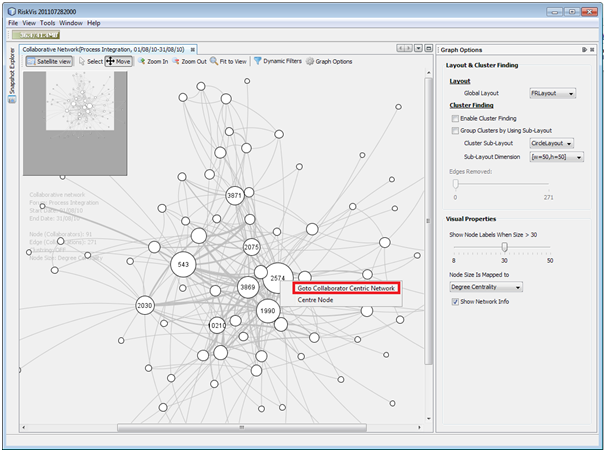
\includegraphics{0a_08}
  \caption{Node 2574's Context Menu.}
  \label{Figure:0a_08}
\end{figure}

\begin{figure}[!htb]
  \centering
  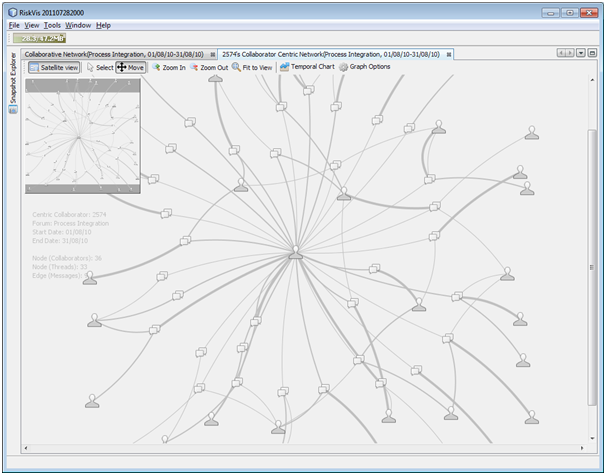
\includegraphics{0a_09}
  \caption{Node 2574's Collaborator-Thread Network.}
  \label{Figure:0a_09}
\end{figure}

\begin{figure}[!htb]
  \centering
  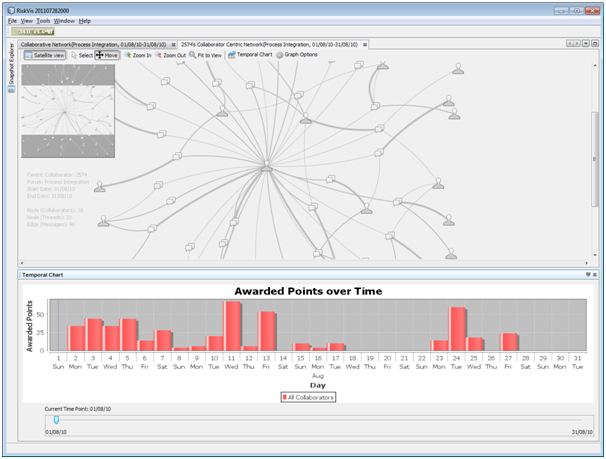
\includegraphics{0a_10}
  \caption{Temporal Chart in Node 2574's Collaborator-Thread Network.}
  \label{Figure:0a_10}
\end{figure}

\begin{figure}[!htb]
  \centering
  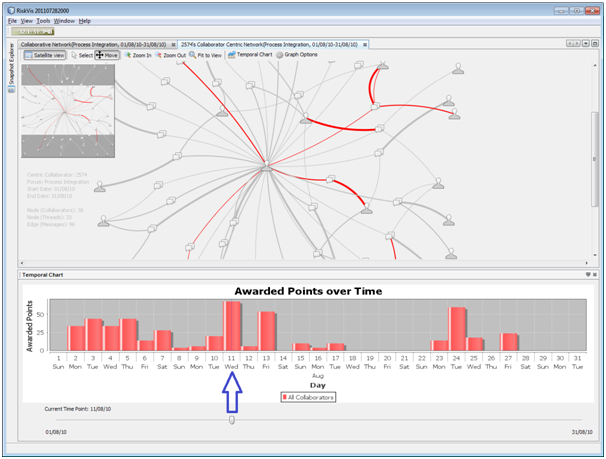
\includegraphics{0a_11}
  \caption{Click Highest Bar in Temporal Chart of Node 2574's Collaborator Centric Network.}
  \label{Figure:0a_11}
\end{figure}

\section{Task D: Find Out Who Can Replace the Most Important Collaborator}
\begin{enumerate}
	\item Suppose you have finished Task A and B, and have realised that the collaborator 2574 is the most important one in the network. Now you are a risk manager, you should do something in preparation for the collaborator 2574's leaving. First of all, you want to find out those collaborators who have the similar knowledge and expertise to replace the collaborator 2574; \\
	\item In \fref{Figure:0a_07}, click the Select toggle button in the top left of the network. Then click the node labelled 2574. As shown in \fref{Figure:0a_12}, the collaborator 2574 is highlighted in yellow while her collaborators are marked in red. Obviously, all collaborators in red may replace the collaborator 2574 to some extent. Now you may wonder who has the most similar knowledge among these candidates; \\
	\item Repeat the Step 1 in Task B to open the `Graph Options' window. Click `Enable Cluster Finding' and `Group Cluster by using Sub-Layout' checkboxes in the red rectangle of \fref{Figure:0a_13}, all nodes are marked with the same colour except the collaborator 2574 as well as his/her collaborators; \\
	\item First click somewhere blank in the network to turn off the highlighting feature. Then drag the knob of the `Edges Removed' slider to the upper bound (value=271) in the red rectangle of \fref{Figure:0a_14}. Now you may gradually decrease the value of the slider to find out the closest collaborator to the node 2574 (HINT: use left arrow key in the keyboard to accurately decrease the value when the slider has got the focus); \\
	\item \fref{Figure:0a_15} shows the status of the network when 267 edges have been removed. You can find there is a dark grey edge between the collaborator 543 and the collaborator 2574. This fact means the former can replace the latter if the latter leaves the forum.
\end{enumerate}

\begin{figure}[!htb]
  \centering
  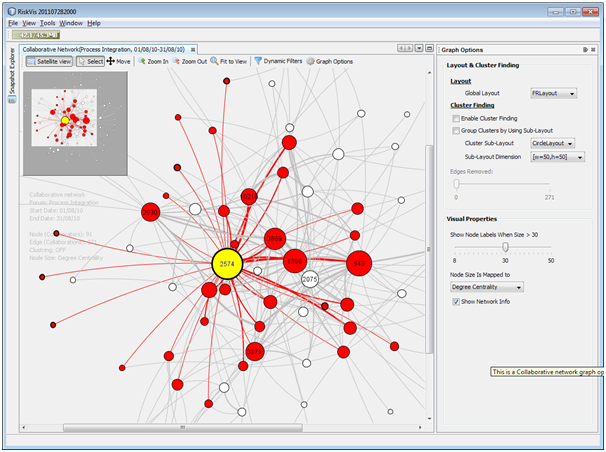
\includegraphics{0a_12}
  \caption{Select Node 2574 in Collaborative Network.}
  \label{Figure:0a_12}
\end{figure}

\begin{figure}[!htb]
  \centering
  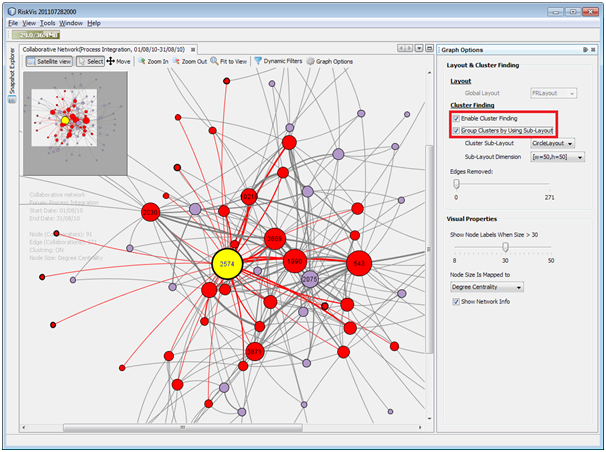
\includegraphics{0a_13}
  \caption{Enable Cluster Finding Functionality in Collaborative Network.}
  \label{Figure:0a_13}
\end{figure}

\begin{figure}[!htb]
  \centering
  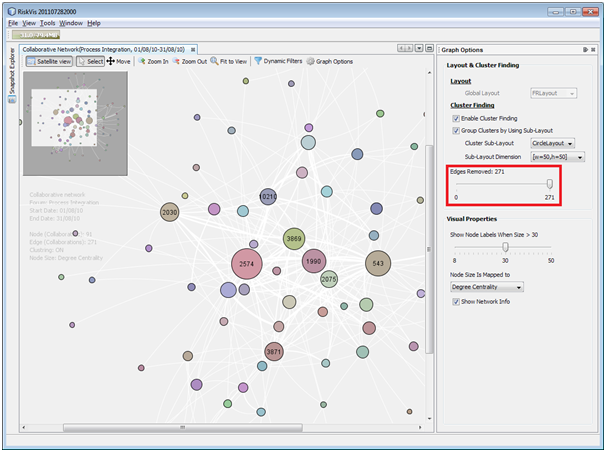
\includegraphics{0a_14}
  \caption{the Status of Collaborative Network after 271 Edges Removed.}
  \label{Figure:0a_14}
\end{figure}

\begin{figure}[!htb]
  \centering
  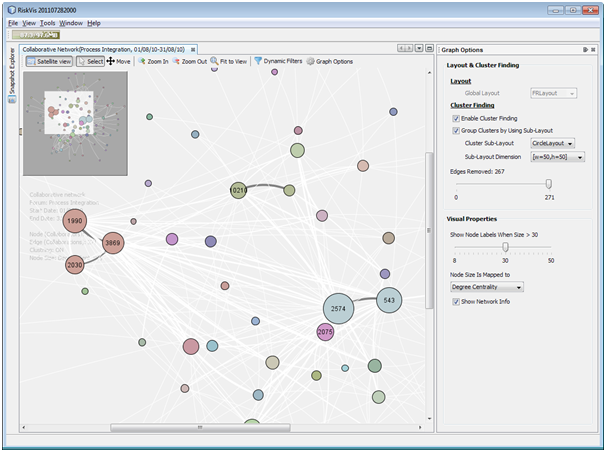
\includegraphics{0a_15}
  \caption{the Status of Collaborative Network after 267 Edges Removed.}
  \label{Figure:0a_15}
\end{figure}